% MDPI Universe manuscript draft using the local MDPI template files in
% paper/Definitions.

\documentclass[universe,article,submit,pdftex,moreauthors]{Definitions/mdpi}

\firstpage{1}
\pubvolume{1}
\issuenum{1}
\articlenumber{0}
\pubyear{2026}
\copyrightyear{2026}
\doinum{}
\hreflink{}
\datereceived{ }
\daterevised{ }
\dateaccepted{ }
\datepublished{ }
\setlength{\headheight}{24.2pt}

\Title{KAN-Payne: A Kolmogorov--Arnold Network Spectral Emulator for Stellar Label Inference}
\TitleCitation{KAN-Payne: A Kolmogorov--Arnold Network Spectral Emulator for Stellar Label Inference}
\Author{Shuo Zhang$^{1}$, Rui Wang $^{2,3}$}
\AuthorNames{Shuo Zhang, Rui Wang}
\AuthorCitation{Zhang, S. \& Wang, R.}
\address{%
$^{1}$ \quad Department of Astronomy, Tsinghua University, Beijing 100084, China
\\
$^{2}$ \quad National Astronomical Observatories, Chinese Academy of Sciences, Beijing 100101, China
\\
$^{3}$ \quad University of Chinese Academy of Sciences, Beijing 100049, China
}
\corres{Correspondence: wangrui@nao.cas.cn}

\abstract{Stellar labels in large spectroscopic surveys are commonly obtained by matching
observed spectra to synthetic grids or by training empirical spectral models on
reference stars. Both strategies depend on a fast representation of the mapping
between stellar labels and flux. We present KAN-Payne, a Payne-style spectral
emulator that replaces the fully connected multilayer perceptron in The Payne
with a Kolmogorov--Arnold Network. Stellar spectra are smooth functions of
atmospheric labels over much of the training domain, while individual
wavelength pixels can have sharply varying responses near temperature- and
abundance-sensitive features. KAN layers, with learnable univariate functions
on network edges, provide a direct way to model such responses. We evaluate
KAN-Payne on the APOGEE-like Kurucz synthetic spectra released with The Payne
and use Payne-MLP and a TransformerPayne-style model as reference baselines.
The benchmark fixes the wavelength grid, pixel mask, label list,
training--validation split, and label scaling, so the comparison focuses on
emulator architecture. On the 10000-epoch synthetic-grid benchmark, KAN-Payne
reaches a validation MAE of 20.89 in units of $10^4$ times the flux residual,
compared with 57.71 for Payne-MLP and 35.18 for the TransformerPayne-style
baseline. The public pretrained Payne MLP reaches 17.44 on the same file and
is retained as an external reference because its training protocol differs. We
then use the trained emulators as differentiable forward models for APOGEE
DR17 spectra. On a common 9117-star quality-controlled sample, KAN-Payne gives
a robust scatter of 113~K in $T_{\mathrm{eff}}$ and 0.053~dex in [Fe/H]
relative to ASPCAP, smaller than the corresponding Payne-MLP and
TransformerPayne-style values for these two labels. The main observed-spectrum
systematic is a positive $\log g$ offset. The paper is organized as a methods
study and emphasizes the accuracy and deployment of KAN-Payne for survey-scale
stellar parameter inference.}

\keyword{stellar spectroscopy; APOGEE; stellar parameters; Kolmogorov--Arnold networks; spectral emulators; machine learning}

\begin{document}

\section{Introduction}

Stellar spectra are one of the main observational links between Galactic
surveys and stellar astrophysics. Effective temperature, surface gravity,
metallicity, and detailed abundance ratios enter distance estimation, age
inference, chemical-tagging studies, selection-function modeling, and the
construction of chemo-dynamical maps of the Milky Way. The scientific value of
large spectroscopic surveys therefore depends not only on the number of spectra,
but also on the reliability and homogeneity of the stellar labels derived from
them. This requirement has shaped the analysis systems of modern surveys such
as APOGEE, LAMOST, GALAH, and RAVE
\cite{majewski2017apogee,abdurrouf2022sdssdr17,luo2015lamostdr1,buder2021galahdr3,kordopatis2013rave}.

Most production pipelines still start from a physically interpretable idea:
compare the observed spectrum with synthetic spectra and find the atmospheric
labels that minimize a spectral residual. APOGEE's ASPCAP performs
pseudo-continuum normalization, fits global stellar parameters with synthetic
model grids, and then derives individual abundances in selected wavelength
windows \cite{garciaperez2016aspcap}. FERRE supplies the grid interpolation and
optimization machinery used by ASPCAP and related analyses
\cite{allendeprieto2015ferre}. LAMOST uses automated low-resolution pipelines
such as LASP and LSP3 to deliver radial velocities and atmospheric parameters
for millions of stars \cite{wu2014lasp,luo2015lamostdr1,xiang2015lsp3}. RAVE
DR4 combined MATISSE and DEGAS for medium-resolution Ca-triplet spectra
\cite{kordopatis2013rave}. GALAH DR3 used Spectroscopy Made Easy with MARCS
model atmospheres, while later GALAH analyses increasingly combine synthetic
spectra with neural-network acceleration \cite{buder2021galahdr3}. These
pipelines are successful because they keep contact with stellar-atmosphere
physics, but their cost grows quickly with the number of labels, wavelength
pixels, and survey spectra.

A second family of methods learns the spectrum--label relation from reference
stars. The Cannon models normalized flux at each wavelength as a flexible
function of stellar labels, enabling label transfer between surveys
\cite{ness2015cannon,ho2017cannon2}. StarNet and astroNN showed that neural
networks can infer APOGEE-like parameters and abundances rapidly from observed
spectra \cite{fabbro2018starnet,leung2019astronn}. SLAM used support-vector
regression for LAMOST spectra, and DD-Payne combined empirical training labels
with Payne-style constraints to estimate abundances for millions of LAMOST
stars \cite{zhang2020slam,xiang2019ddpayne}. These approaches are practical and
fast, but their calibration is tied to the reference set: outside the training
domain, extrapolation and inherited label systematics become central concerns.

The Payne occupies a useful middle ground. It trains a neural emulator on
synthetic spectra, then uses the differentiable emulator as a forward model for
observed spectra \cite{ting2019payne}. This keeps the model anchored to a
physical spectral grid while avoiding repeated high-dimensional interpolation
during fitting. TransformerPayne recently introduced a wavelength-conditioned
transformer emulator and showed that attention-based models can improve
emulation accuracy and data efficiency in synthetic-grid tests
\cite{rozanski2024transformerpayne}. The remaining question is whether there is
a simpler vector-output architecture that keeps the deployment advantages of
The Payne while improving over the standard multilayer perceptron.

This paper introduces KAN-Payne, a Payne-style spectral emulator based on
Kolmogorov--Arnold Networks. KANs replace fixed node activations with learnable
univariate functions on network edges \cite{liu2024kan}. For stellar spectra
this is a natural parameterization: the flux response to atmospheric labels is
smooth over much of the grid, but individual pixels can change sharply near
temperature-sensitive molecular bands or abundance-sensitive atomic lines.
KAN-Payne therefore targets a specific niche. It is not proposed as a universal
replacement for survey pipelines or for transformer models. Instead, it is
designed as a full-spectrum, differentiable emulator that can be dropped into a
Payne-like fitting loop.

This work first formulates KAN-Payne as a vector-output KAN spectral emulator
for Payne-style stellar label inference. It then builds a controlled benchmark
on the public Payne APOGEE/Kurucz synthetic training set, with the wavelength
grid, label scaling, validation split, and pixel mask held fixed across all
models. Under this matched setup, KAN-Payne is compared with Payne-MLP and
TransformerPayne-style baseline through training curves, validation residual
distributions, and wavelength-resolved residuals. The same emulators are
finally used in an APOGEE DR17 parameter-inference experiment, where fitted
labels from observed spectra are compared with the official ASPCAP catalog.

\section{Data}

\subsection{The Payne Synthetic Spectral Grid}

The emulator benchmark uses the Kurucz APOGEE-like synthetic spectra released
with The Payne GitHub repository \cite{ting2019payne}. The file contains 1000
continuum-normalized spectra on the Payne APOGEE wavelength grid. After loading
the public wavelength and mask files, the working grid has 7214 pixels from
15168.13 to 16936.75~\AA. The target vector for each spectrum contains 25
labels: $T_{\mathrm{eff}}$, $\log g$, microturbulence, 19 elemental abundance
labels, $^{12}$C/$^{13}$C, and macroturbulence. We keep the repository split:
800 spectra for training and 200 spectra for validation. Pixels marked by the
Payne APOGEE mask are excluded from the primary validation metric, but they are
kept in the arrays so that all models return spectra on the same grid.

The labels are scaled using training-set bounds,
\begin{equation}
    \label{eq:label-scaling}
    \tilde{\ell}_i =
    \frac{\ell_i - \ell_{i,\min}}{\ell_{i,\max}-\ell_{i,\min}} - 0.5,
\end{equation}
which maps the training range to approximately $[-0.5,0.5]$. The spectra are
used in their continuum-normalized flux units. For the vector-output models,
the loss is computed across the full 7214-pixel vector. For the
TransformerPayne-style baseline, wavelengths are additionally scaled to
$[-1,1]$ because the model predicts flux as a function of labels and
wavelength.

\subsection{APOGEE DR17 Spectra and ASPCAP Labels}

The observed-spectra experiment uses APOGEE DR17 \texttt{aspcapStar} products
and the official \texttt{allStar-dr17-synspec\_rev1} catalog. APOGEE observes
near-infrared H-band spectra at a resolving power of approximately 22500 over
1.51--1.70~$\mu$m \cite{majewski2017apogee,wilson2019apogee}. DR17 is the final
SDSS-IV release and includes the completed APOGEE-2 data set
\cite{abdurrouf2022sdssdr17}. ASPCAP provides the comparison labels used here:
calibrated $T_{\mathrm{eff}}$, $\log g$, [M/H], [Fe/H], [$\alpha$/M], and
selected abundance ratios \cite{garciaperez2016aspcap,jonsson2020apogeedr16}.

We select a conservative red-giant clean sample from the DR17 catalog. The
selection requires finite ASPCAP labels, no severe ASPCAP or stellar warning
flags, at least two visits, APOGEE spectra from either the APO or LCO
telescope, $3500<T_{\mathrm{eff}}<5500$~K, $0<\log g<3.8$,
$-2.0<\mathrm{[Fe/H]}<0.5$, and \texttt{SNREV}$>100$. The current analysis
sample contains 10000 stars. Its median ASPCAP labels are
$T_{\mathrm{eff}}=4658$~K, $\log g=2.39$, and $\mathrm{[Fe/H]}=-0.23$. The
median per-star S/N estimated from the normalized flux and uncertainty arrays
is 137.

\subsection{Observed-Spectrum Preprocessing}

We work with \texttt{aspcapStar} spectra rather than raw visit spectra. These
files are already combined, shifted to the stellar rest frame, and supplied with
the APOGEE pseudo-continuum normalization. However, direct use of the
\texttt{aspcapStar} flux leaves chip-scale continuum residuals that are not well
matched to the Payne synthetic spectra. We therefore follow the normalization
strategy used in The Payne fitting code for APOGEE spectra: after interpolation
onto the Payne wavelength grid, a fourth-order Chebyshev continuum is fitted
separately on the blue, green, and red APOGEE detector segments using a fixed
set of continuum pixels. In the absence of the original binary continuum-pixel
file, we rebuild an equivalent mask from the public Payne synthetic grid by
selecting, within each detector segment, pixels with median synthetic flux
closest to unity and low object-to-object variance. The same continuum-pixel
mask is then used for every APOGEE spectrum.

The preprocessing begins by downloading the selected \texttt{aspcapStar} files
from the SDSS DR17 SAS tree. For each FITS file we read the normalized flux,
uncertainty, best-fit ASPCAP model, and wavelength solution from the image
HDUs. A 0.005 floor in normalized-flux units is added to the flux uncertainty
before fitting so that individual pixels with very small formal errors do not
dominate the likelihood. Flux and
uncertainty are then resampled from the 8575-pixel APOGEE
\texttt{aspcapStar} grid to the 7214-pixel Payne grid by one-dimensional
interpolation. After resampling, the three-chip Chebyshev continuum described
above is fitted and divided out using identical continuum pixels for the full
sample. The final fitting mask combines the APOGEE bad-pixel mask, non-finite
values, non-positive uncertainties, and the Payne pixel mask.
The median number of usable Payne-grid pixels per star after masking is 6339,
about 87.9\% of the 7214-pixel grid. The continuum-pixel mask contains 576
pixels, distributed as 233, 192, and 151 pixels across the three APOGEE
detector segments. This step changes only the smooth continuum scale; the
line-level mask and ASPCAP labels are unchanged.

\begin{figure}[H]
\centering
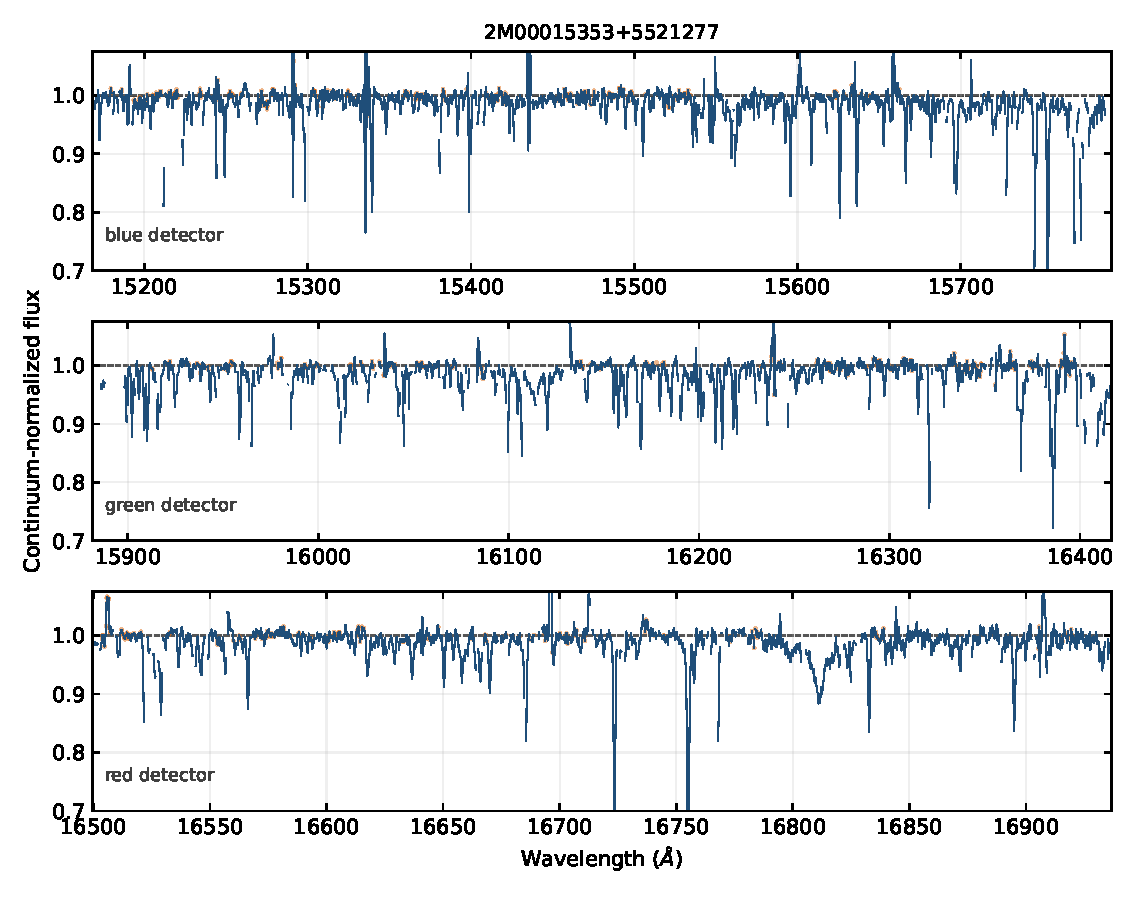
\includegraphics[width=0.9\linewidth]{figures/apogee_sample_spectrum.pdf}
\caption{Example APOGEE DR17 \texttt{aspcapStar} spectrum after interpolation
onto the Payne wavelength grid and Payne-style three-chip Chebyshev continuum
renormalization. The three panels show the blue, green, and red APOGEE detector
segments separately so that detector gaps are not connected by the plotted
line. Orange markers indicate the fixed continuum pixels used for the
Chebyshev fit.}
\label{fig:apogee-sample-spectrum}
\end{figure}

\section{Methods}

\subsection{Payne-MLP Baseline}

The Payne-MLP baseline maps the 25 scaled stellar labels directly to the full
7214-pixel spectrum through two hidden layers. We reproduce the original
GitHub-released pretrained Payne network with a NumPy forward pass and train a
new MLP under the same unified split for a controlled comparison.

For the controlled run the network has two hidden layers with 300 neurons each.
The activation function is a LeakyReLU with negative slope 0.01. The model is
trained with a mean absolute flux loss,
\begin{equation}
    \label{eq:mlp-loss}
    \mathcal{L}_{\mathrm{MLP}} =
    \frac{1}{N_{\mathrm{batch}}N_{\mathrm{pix}}}
    \sum_{n,p} | f_{n,p}^{\mathrm{pred}} - f_{n,p}^{\mathrm{true}} |,
\end{equation}
using raw continuum-normalized fluxes rather than per-pixel normalized targets.
Validation is reported in units of $10^4$ times the flux residual. The formal
10000-epoch run uses AdamW with learning rate $10^{-4}$, zero weight decay, no
target-spectrum normalization, and the best checkpoint selected by validation
MAE on unmasked Payne pixels. The Payne-MLP uses batch size 128. KAN-Payne and
the TransformerPayne-style baseline use the same optimizer settings with batch
sizes 64 and 32, respectively, chosen to keep the A100 training jobs stable.

\subsection{KAN-Payne: Proposed Emulator}

KAN-Payne replaces the MLP layers with a vector-output KAN emulator. The model
uses the same input labels, target spectra, loss function, and validation split
as Payne-MLP. This isolates the effect of the KAN architecture from data and
preprocessing choices.

The architectural difference from a standard MLP is easiest to see at the
level of one layer. In an MLP, each hidden unit first forms a linear mixture of
the previous activations and then applies a fixed scalar nonlinearity,
\begin{equation}
    \label{eq:mlp-layer}
    \mathbf{h}^{(l+1)} =
    \sigma\!\left(\mathbf{W}^{(l)}\mathbf{h}^{(l)}+\mathbf{b}^{(l)}\right),
\end{equation}
where the trainable part is the affine map and the activation function
$\sigma$ is fixed in advance. This design is expressive and computationally
efficient, but all nonlinear structure must be assembled by combining many
fixed activations. A KAN layer instead assigns a learnable univariate function
to each edge between input and output coordinates,
\begin{equation}
    \label{eq:kan-layer}
    h^{(l+1)}_j =
    \sum_i \phi^{(l)}_{j i}\!\left(h^{(l)}_i\right),
\end{equation}
where the functions $\phi^{(l)}_{ji}$ are trainable. In practice these edge
functions are represented by a smooth basis expansion together with a simple
base activation. The model therefore learns not only how strongly one label
coordinate contributes to the next representation, but also the shape of that
one-dimensional response.

This distinction is important for stellar spectra. The flux at a given pixel is
often a smooth but non-linear function of $T_{\mathrm{eff}}$, $\log g$, and
abundance labels. The response can be nearly monotonic in continuum regions,
change rapidly near ionization or molecular-equilibrium transitions, and become
locally saturated in strong absorption lines. An MLP can model these effects,
but it does so through repeated affine mixing followed by fixed nonlinearities.
KAN-Payne gives each edge a flexible response curve, which is a more direct
parameterization for the smooth one-dimensional label dependencies that appear
throughout a synthetic spectral grid. The summation over learned edge functions
also keeps the model differentiable with respect to the input labels, which is
required by the downstream Payne-style fitting step.

The adopted architecture is
\begin{equation}
    \label{eq:kan-architecture}
    25 \rightarrow 64 \rightarrow 256 \rightarrow 7214 ,
\end{equation}
with GELU base activations in the KAN layers. The implementation uses the
efficient-kan edge-function parameterization, in which each edge
function combines a cubic spline component and a base activation. We use
\texttt{grid\_size}=5, \texttt{spline\_order}=3, the default
efficient-kan noise and spline scaling, and GELU as the base
activation. The input dimension is the
25 scaled Payne labels, and the output dimension is the full 7214-pixel
APOGEE-like spectrum. We use a vector-output design rather than training one
independent model per wavelength pixel. This couples the pixel predictions
through shared hidden representations and allows a single forward pass to
produce the entire spectrum. The architecture is not meant to be the final
architecture search for KANs; rather, it is a practical configuration that can
be trained repeatedly while preserving enough capacity to model thousands of
APOGEE pixels.

KAN-Payne keeps the main advantages of The Payne formulation. It predicts the
whole spectrum in one forward pass, it is differentiable with respect to the
stellar labels, and it can therefore be used directly inside gradient-based
spectral fitting. Its distinction from Payne-MLP lies in the parameterization of
the label--flux function: instead of relying only on affine transformations and
fixed pointwise activations, each KAN layer learns edge functions whose shapes
can adapt to the training grid.
Compared with wavelength-conditioned TransformerPayne-style models, KAN-Payne
does not explicitly condition on wavelength and therefore lacks the
transformer's long-range attention mechanism, but it is simpler to deploy in a
full-spectrum fitting loop because it retains vector-output behavior. In this
work, KAN-Payne is therefore treated as a vector-output alternative to the
original Payne-MLP: more adaptive than a fixed-activation MLP, but still close
to The Payne in how it is called during spectral fitting.

\subsection{TransformerPayne-Style Baseline}

Our TransformerPayne-style baseline is implemented as a wavelength-conditioned
scalar-flux model.
It encodes the label vector into learned label tokens and encodes the requested
wavelength with sinusoidal features. Cross-attention blocks condition wavelength
queries on the label tokens, and a small regression head predicts the flux at
the requested wavelength. During training we sample wavelength pixels for each
spectrum; during validation we scan the full 7214-pixel grid in chunks.
This implementation follows the main architectural idea of TransformerPayne
but is trained inside the same data loader, optimizer schedule, and validation
framework as the MLP and KAN models. It should therefore be read as a local
TransformerPayne-style comparison rather than a claim about every possible
tuning of the published TransformerPayne code.

For the main experiment the label vector is mapped to 16 tokens of width 128.
The wavelength coordinate is scaled to $[-1,1]$ and expanded with sinusoidal
features. Four cross-attention blocks with four attention heads update the
wavelength query against the label tokens. At each training step, 256 wavelength
pixels are sampled per spectrum. This sampling scheme makes the scalar-output
model compatible with the same validation protocol while still evaluating the
full spectrum during validation.

\subsection{APOGEE Parameter Inference}

For each observed APOGEE spectrum we optimize the 25 scaled Payne labels by
minimizing an uncertainty-weighted residual objective,
\begin{equation}
    \label{eq:apogee-objective}
    \chi^2_{\mathrm{red-like}}(\boldsymbol{\ell}) =
    \frac{1}{N_{\mathrm{pix}}}
    \sum_{p \in \mathcal{P}}
    \left[
    \frac{f^{\mathrm{obs}}_p -
    f^{\mathrm{emu}}_p(\boldsymbol{\ell})}{\sigma_p}
    \right]^2,
\end{equation}
where $\mathcal{P}$ excludes masked Payne pixels and bad observed pixels. The
normalization by $N_{\mathrm{pix}}$ makes this a reduced-chi-square-like
objective rather than a formally calibrated reduced $\chi^2$, because the
continuum-normalized pixels have correlated errors and an imposed uncertainty
floor.
ASPCAP labels initialize $T_{\mathrm{eff}}$, $\log g$, and [Fe/H] when
available; other labels start from the training-grid midpoint unless an ASPCAP
abundance proxy is available. The fitted labels are then compared against
ASPCAP calibrated parameters.

\section{Results}

\subsection{Synthetic Emulator Benchmark}

All emulator comparisons use the same 800/200 synthetic split. We report MAE
and RMSE in units of flux residuals multiplied by $10^4$, both over all pixels
and over unmasked Payne pixels. The pretrained Payne-MLP released with The
Payne gives a validation MAE of 17.44 and RMSE of 68.31 on unmasked pixels for
this repository benchmark. This pretrained model is not a controlled baseline
because its training details and stopping point differ from our run; it is kept
as an external reference to check that the data loader and wavelength grid are
consistent with the public Payne release.

The validation figures follow the convention used in survey-pipeline and
spectral-emulator papers: a scalar summary table is not sufficient by itself.
We therefore use four complementary views. The first is the training history,
which shows whether a model has reached a stable validation floor or is still
improving. The second is the residual histogram over all validation spectra and
unmasked pixels, which makes non-Gaussian tails visible. The third is the
wavelength-resolved residual curve, which shows whether an emulator fails
globally or only near specific spectral features. The fourth is a star-by-star
residual summary, used to identify whether a small subset of validation spectra
dominates the metric. This style follows the logic of ASPCAP validation,
The Payne emulator tests, and neural-network label-transfer studies: scalar
precision, systematic residuals, and outlier structure are reported together
\cite{garciaperez2016aspcap,ting2019payne,fabbro2018starnet,leung2019astronn}.

\begin{table}[H]
\centering
\caption{Synthetic validation performance. KAN-Payne is the proposed method;
Payne-MLP and the TransformerPayne-style emulator define the local comparison
baseline. The
trainable-model rows use the best validation checkpoints from the 10000-epoch
A100 run.}
\label{tab:synthetic-validation}
\begin{tabular}{lrrrr}
\toprule
Model & Epoch & MAE$_{\mathrm{good}}$ & RMSE$_{\mathrm{good}}$ & Notes \\
\midrule
Payne pretrained MLP & -- & 17.44 & 68.31 & GitHub coefficients \\
Payne-MLP & 9933 & 57.71 & 106.81 & best 10k checkpoint \\
KAN-Payne & 9964 & 20.89 & 57.12 & best 10k checkpoint \\
TransformerPayne-style & 9932 & 35.18 & 86.94 & best 10k checkpoint \\
\bottomrule
\end{tabular}
\end{table}

\begin{figure}[H]
\centering
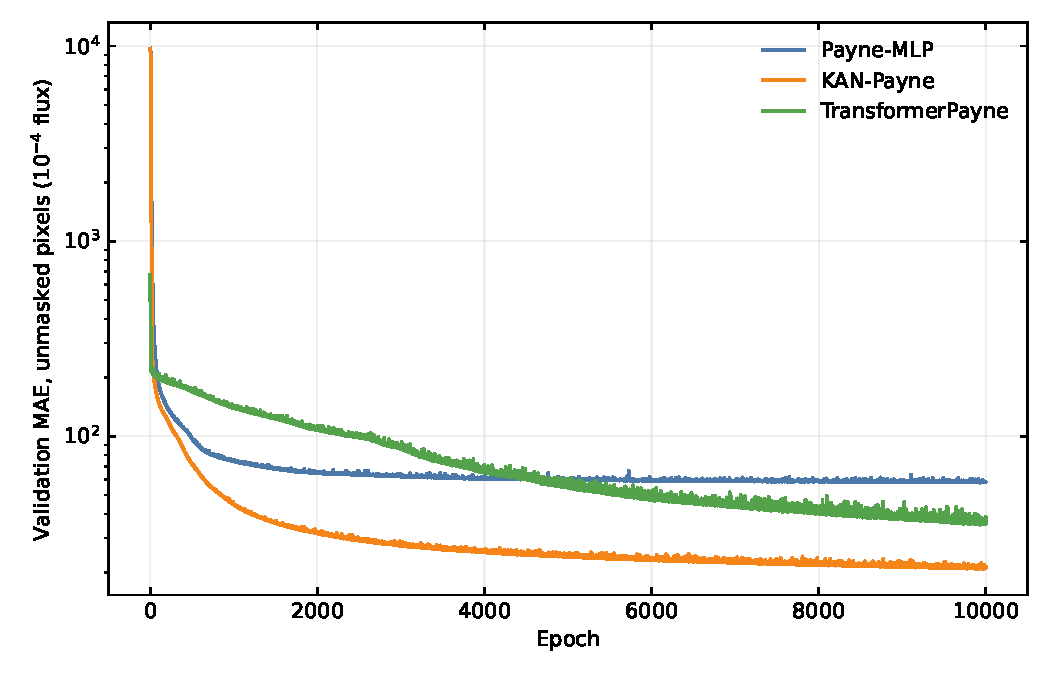
\includegraphics[width=0.72\linewidth]{figures/validation_mae_history.pdf}
\caption{Validation MAE on unmasked Payne pixels as a function of training
epoch. KAN-Payne reaches the lowest validation floor among the three controlled
emulator runs.}
\label{fig:validation-history}
\end{figure}

\begin{figure}[H]
\centering
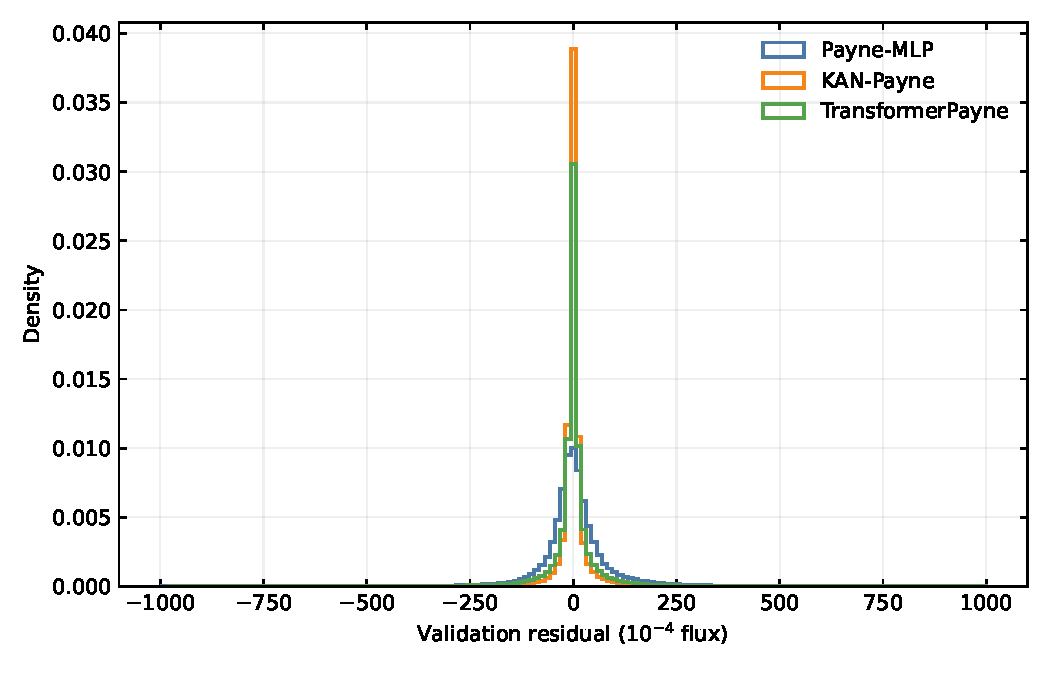
\includegraphics[width=0.72\linewidth]{figures/synthetic_residual_histogram.pdf}
\caption{Distribution of validation residuals over all validation spectra and
unmasked Payne pixels. KAN-Payne narrows the residual core relative to the
controlled Payne-MLP and TransformerPayne-style runs.}
\label{fig:synthetic-residual-histogram}
\end{figure}

\begin{figure}[H]
\centering
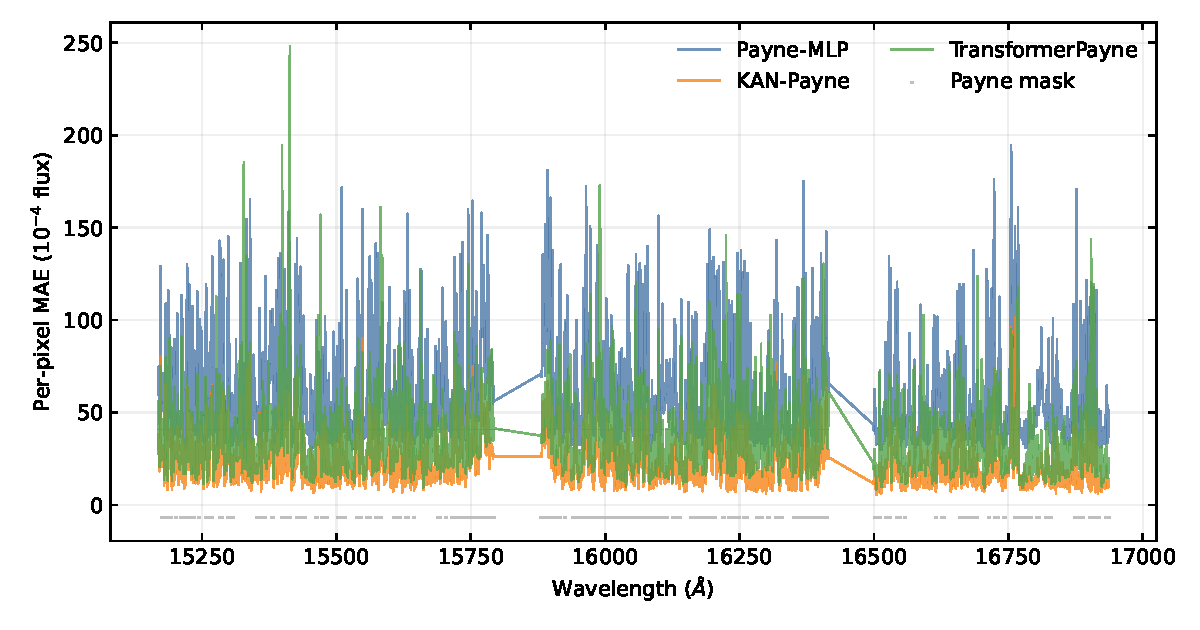
\includegraphics[width=0.72\linewidth]{figures/pixel_residual_summary.pdf}
\caption{Per-pixel validation residuals for Payne-MLP, KAN-Payne, and the
TransformerPayne-style baseline. The plot highlights wavelength regions where
emulator errors are concentrated.}
\label{fig:pixel-residuals}
\end{figure}

KAN-Payne reaches a validation MAE of 20.89 and RMSE of 57.12 on unmasked
Payne pixels. Under the same split and flux target, Payne-MLP reaches 57.71
and 106.81, while the TransformerPayne-style baseline reaches 35.18 and 86.94.
KAN-Payne therefore reduces the MAE by 63.8\% relative to Payne-MLP and by
40.6\% relative to the TransformerPayne-style baseline in this synthetic
validation experiment. The wavelength-resolved plot shows that the improvement
is not confined to a single small spectral interval; KAN-Payne lowers the
residual level across much of the Payne grid, while the largest remaining
errors still occur near strong and blended spectral features. The pretrained
Payne MLP remains the best absolute reference on this public 1000-spectrum
file under the original Payne training protocol, so the claim made here is
restricted to the controlled local training protocol.

\subsection{APOGEE DR17 Stellar Parameter Inference}

The APOGEE DR17 experiment asks whether the synthetic-emulator ranking carries
over to observed spectra. We fit the same 10000-star clean sample with
Payne-MLP, KAN-Payne, and the TransformerPayne-style baseline. For each
spectrum we optimize the 25 scaled Payne labels by minimizing the
uncertainty-weighted residual objective in Equation~\eqref{eq:apogee-objective}.
The fit uses 2048 good pixels sampled without replacement for optimization; the
sampling uses a global random seed of 42, is repeated identically for the three
emulators, and is held fixed for each star during its 600 Adam optimization
steps. The final residual is then evaluated on all unmasked pixels.
ASPCAP values initialize $T_{\mathrm{eff}}$, $\log g$, [Fe/H], and the
available abundance proxies; labels without an ASPCAP proxy start at the center
of the synthetic training range. Each model is fitted from its best
10000-epoch synthetic-validation checkpoint.

The reported APOGEE metrics are the median residual, the robust scatter
$1.4826\,\mathrm{MAD}$, and the 16th--84th percentile interval of
fit--ASPCAP residuals for $T_{\mathrm{eff}}$, $\log g$, and [Fe/H]. We also
track the median spectral fit MAE and $\chi^2_{\mathrm{red-like}}$ because a
model can agree with ASPCAP labels while still fitting the normalized spectrum
poorly. All three models successfully return labels for all 10000 spectra. For
the atmospheric
comparison we require at least 5000 valid pixels, reject the upper 1\% tail in
model-specific $\chi^2_{\mathrm{red-like}}$ and spectral MAE, and require the
three atmospheric labels to remain inside the scaled training interval. These
model-specific quality cuts keep 9244 Payne-MLP stars, 9526 KAN-Payne stars,
and 9408 TransformerPayne-style stars. To avoid comparing different stellar
samples, the reported residual table and the main APOGEE figures use the
intersection of the three quality masks, containing 9117 stars. On this common
sample the median spectral MAE values are 148.7, 147.4, and 166.3 in units of
$10^4$ times the flux residual for Payne-MLP, KAN-Payne, and the
TransformerPayne-style baseline, respectively. The spectral MAE values for
Payne-MLP and KAN-Payne are therefore close, while their atmospheric residual
scatters differ more strongly. This is expected because the fit objective sums
over thousands of continuum-normalized pixels, whereas the reported labels are
most sensitive to particular temperature-, gravity-, and metallicity-sensitive
features.

The same conclusion holds on the model-specific quality samples. The own-sample
$T_{\mathrm{eff}}$/[Fe/H] scatters are 125.5~K/0.0888~dex for Payne-MLP,
113.3~K/0.0534~dex for KAN-Payne, and 137.4~K/0.0615~dex for the
TransformerPayne-style baseline, close to the corresponding common-sample
values in Table~\ref{tab:apogee-inference}. Thus, the common-sample
intersection does not artificially create the KAN-Payne advantage by selecting
only stars that are easy for all three emulators.

\begin{table}[H]
\centering
\small
\caption{APOGEE DR17 atmospheric-label comparison against ASPCAP on the common
9117-star quality-controlled sample. Residuals are defined as fitted label
minus ASPCAP label. The scatter column gives $1.4826\,\mathrm{MAD}$.}
\label{tab:apogee-inference}
\begin{tabular}{llrrrr}
\toprule
Model & Label & $N$ & Median & $1.4826\,\mathrm{MAD}$ & P16--P84 \\
\midrule
Payne-MLP & $T_{\mathrm{eff}}$ (K) & 9117 & -62.9 & 124.8 & -182.0--78.0 \\
KAN-Payne & $T_{\mathrm{eff}}$ (K) & 9117 & -17.4 & 112.9 & -120.9--108.2 \\
TransformerPayne-style & $T_{\mathrm{eff}}$ (K) & 9117 & -47.1 & 136.4 & -193.5--83.8 \\
Payne-MLP & $\log g$ (dex) & 9117 & 0.105 & 0.222 & -0.122--0.330 \\
KAN-Payne & $\log g$ (dex) & 9117 & 0.197 & 0.199 & 0.000--0.418 \\
TransformerPayne-style & $\log g$ (dex) & 9117 & 0.173 & 0.193 & -0.027--0.372 \\
Payne-MLP & [Fe/H] (dex) & 9117 & 0.048 & 0.088 & -0.032--0.152 \\
KAN-Payne & [Fe/H] (dex) & 9117 & 0.037 & 0.053 & -0.015--0.095 \\
TransformerPayne-style & [Fe/H] (dex) & 9117 & 0.035 & 0.061 & -0.020--0.105 \\
\bottomrule
\end{tabular}
\end{table}

KAN-Payne shows the smallest robust scatter in $T_{\mathrm{eff}}$ and [Fe/H]
and also keeps the largest model-specific atmospheric-quality sample before the
intersection cut. On the common sample its [Fe/H] scatter is 0.053~dex,
compared with 0.088~dex for Payne-MLP and 0.061~dex for the
TransformerPayne-style baseline. The
$T_{\mathrm{eff}}$ scatter is 113~K for KAN-Payne, 125~K for Payne-MLP, and
136~K for the TransformerPayne-style baseline. The main remaining systematic is
a positive
$\log g$ offset of 0.20~dex, slightly larger than the Payne-MLP offset and
comparable to the TransformerPayne-style baseline. This offset is expected to
be sensitive to
continuum placement, the adopted giant-star selection, and the fact that all
three fits optimize the full 25-label Payne vector although only three
atmospheric labels are reported here.

\begin{figure}[H]
\centering
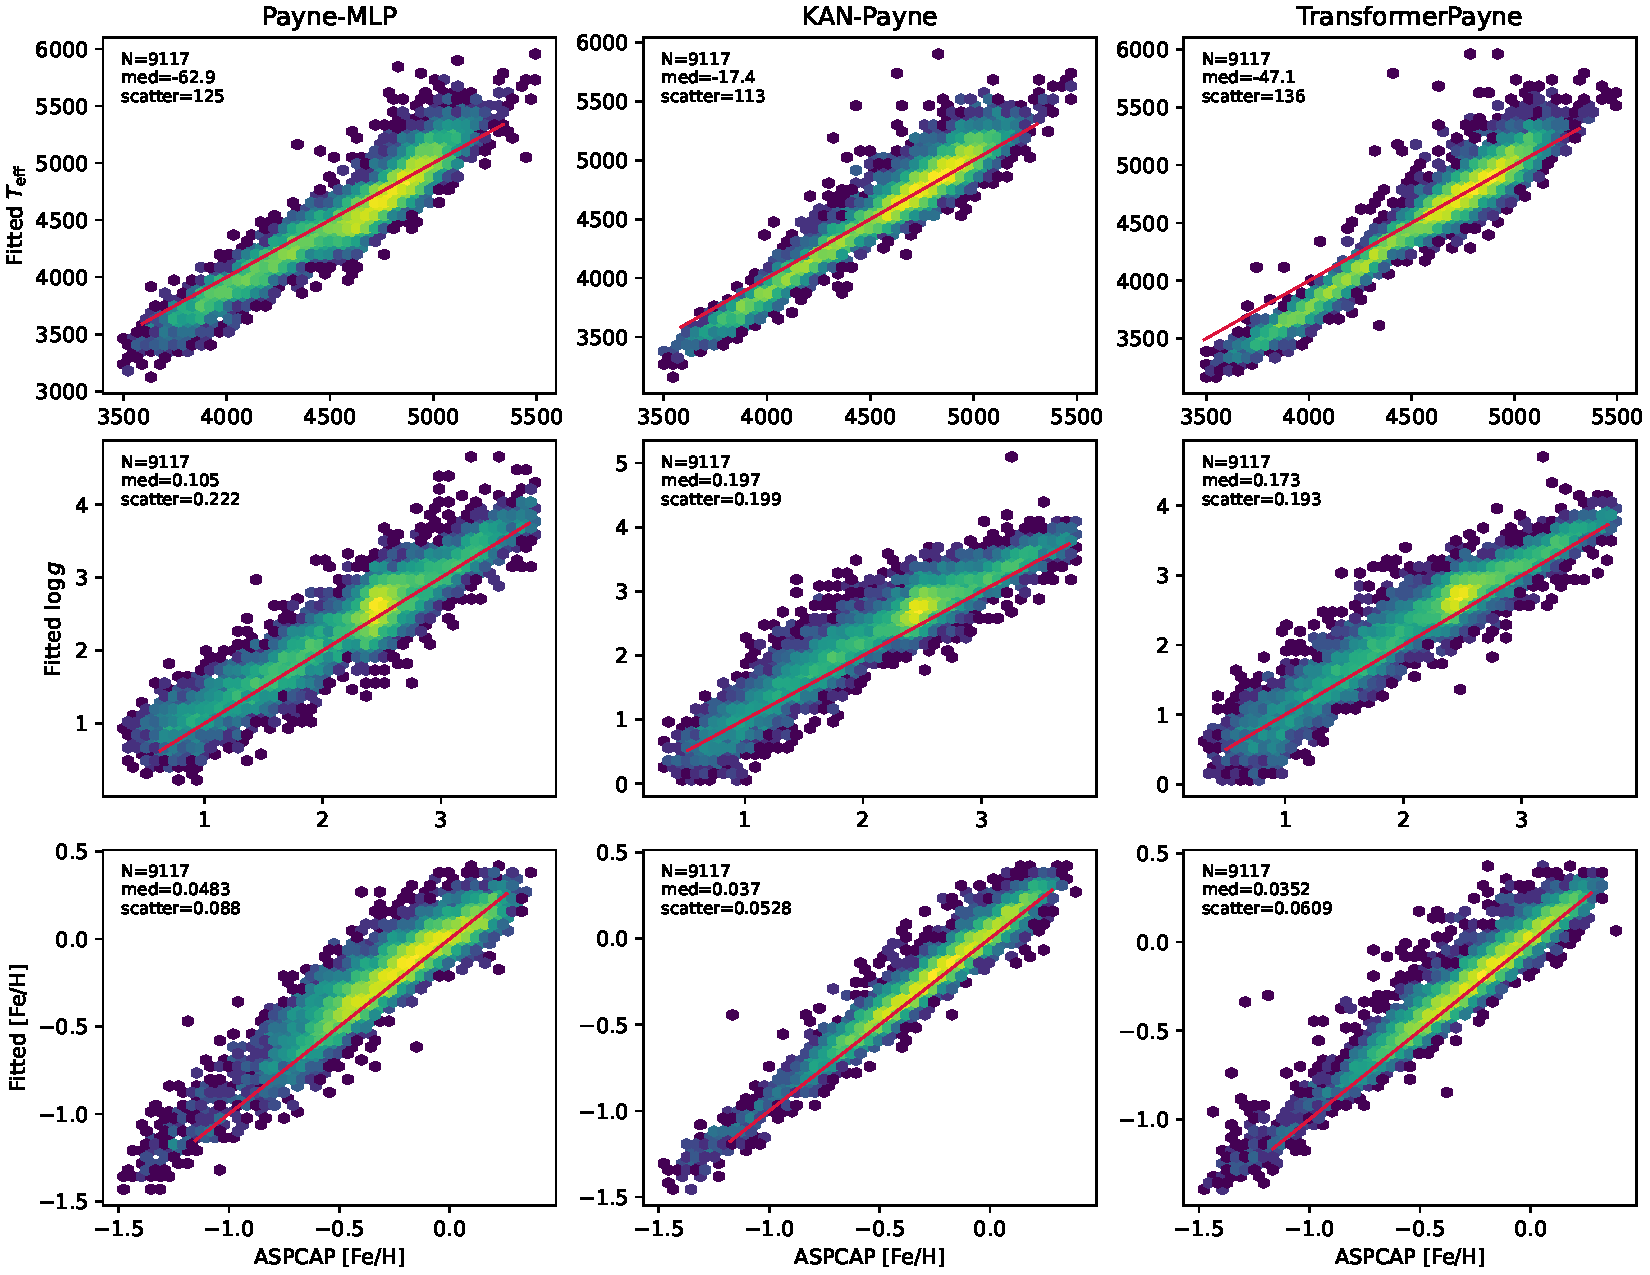
\includegraphics[width=0.95\linewidth]{figures/apogee_inference_10k_payne_norm/apogee_common_aspcap_hexbin_grid.pdf}
\caption{APOGEE DR17 atmospheric-label comparison with ASPCAP. Each column
shows one emulator and each row shows one reported atmospheric label, using the
same 9117-star common quality sample as Table~\ref{tab:apogee-inference}. The
red line marks the one-to-one relation.}
\label{fig:apogee-comparison}
\end{figure}

\begin{figure}[H]
\centering
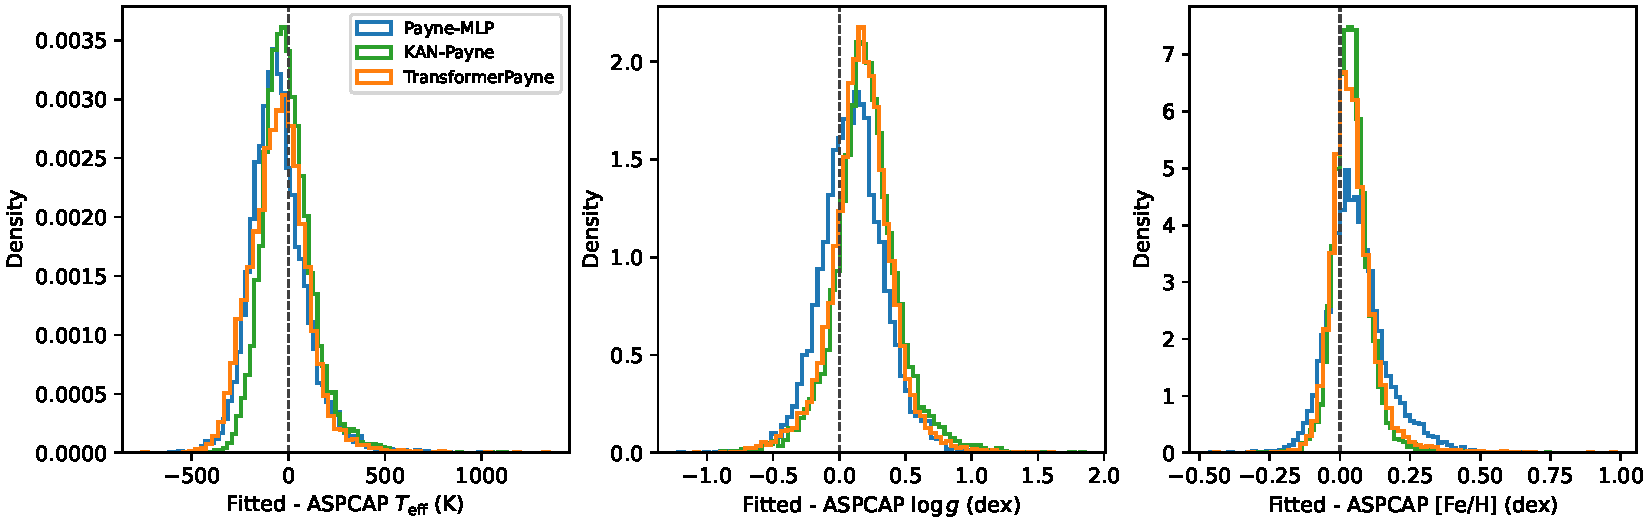
\includegraphics[width=0.95\linewidth]{figures/apogee_inference_10k_payne_norm/apogee_common_residual_distribution.pdf}
\caption{APOGEE DR17 residual distributions for the atmospheric labels. The
narrower KAN-Payne [Fe/H] distribution is consistent with the synthetic-grid
validation result and indicates that the KAN emulator improves the forward
model in abundance-sensitive spectral regions on the common quality sample.}
\label{fig:apogee-residual-distribution}
\end{figure}

\begin{figure}[H]
\centering
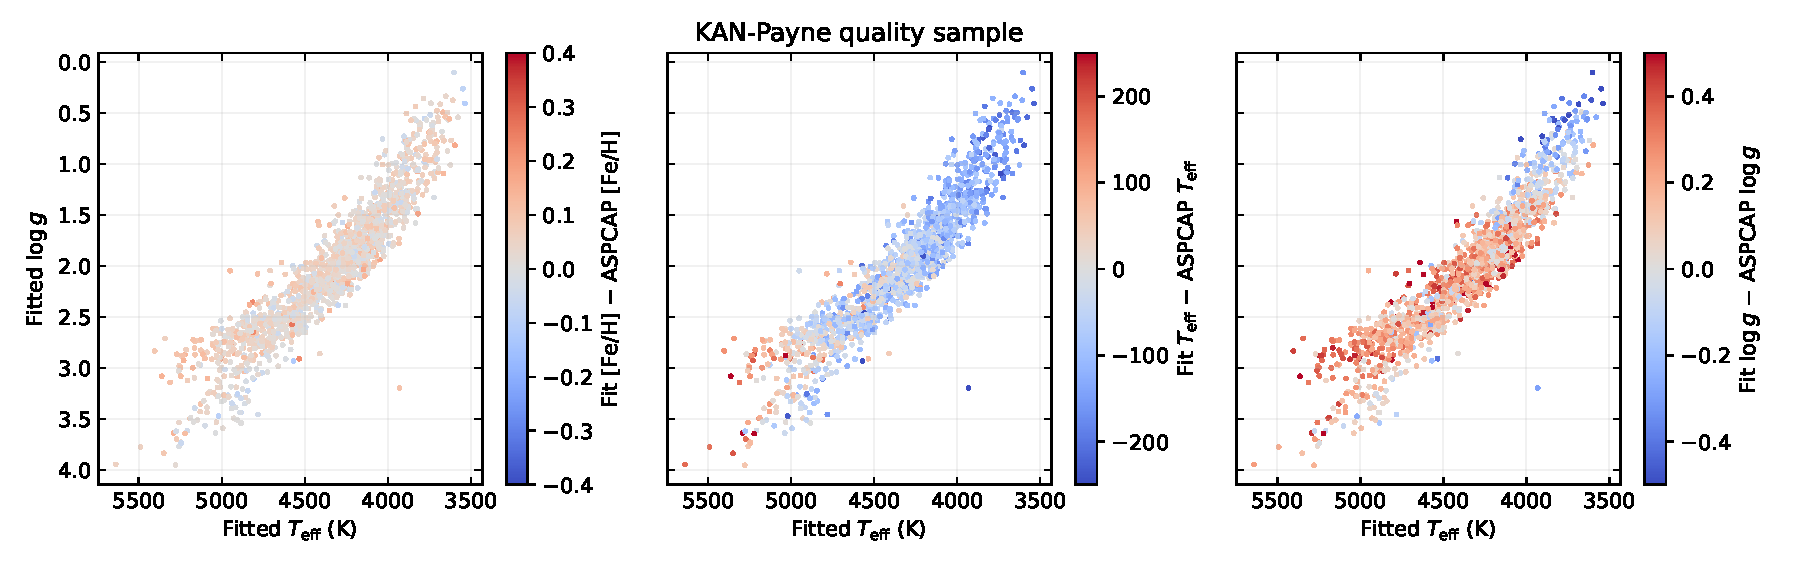
\includegraphics[width=0.85\linewidth]{figures/apogee_inference_10k_payne_norm/apogee_kiel_systematics.pdf}
\caption{KAN-Payne APOGEE DR17 Kiel-diagram residual diagnostics. The panels
show the clean red-giant sample in the ASPCAP $T_{\mathrm{eff}}$--$\log g$
plane and color the same stars by fitted-minus-ASPCAP residuals in [Fe/H],
$T_{\mathrm{eff}}$, and $\log g$. The color limits are
$\pm 0.4$~dex, $\pm 250$~K, and $\pm 0.5$~dex, respectively.}
\label{fig:apogee-kiel}
\end{figure}

\section{Discussion}

This benchmark separates emulator accuracy from downstream label inference.
KAN-Payne is designed for the part of the problem where The Payne is already
attractive: repeated differentiable full-spectrum evaluations in a
moderate-dimensional label space. Its main competitor in that setting is the
Payne-MLP. TransformerPayne-style emulators address a related but not identical
trade-off: they model flux as a function of labels and wavelength and can
exploit long-range correlations, but validation and fitting require scanning
wavelength chunks.
The comparison is therefore not a single ranking of neural architectures. It
identifies which architecture is preferable for a specific survey task:
full-spectrum fitting, wavelength-conditioned scalar emulation, or direct
compatibility with existing Payne workflows.

The controlled synthetic benchmark is the cleanest evidence for the KAN-Payne
architecture. All three trainable models see the same 800 training spectra, 200
validation spectra, label scaling, wavelength grid, and loss definition. Under
these conditions KAN-Payne reduces the validation MAE by 63.8\% relative to the
controlled Payne-MLP and by 40.6\% relative to the TransformerPayne-style
baseline. The public pretrained Payne MLP still gives the lowest synthetic
validation MAE on this exact file, so it is retained as an external reference
rather than treated as a controlled baseline. The controlled comparison in this
paper is therefore deliberately narrower: it asks how the local KAN, MLP, and
TransformerPayne-style implementations behave when the data loader, split,
label scaling, target spectra, and optimization setup are held fixed.

The APOGEE experiment is a more demanding test because the synthetic and
observed spectra do not share the same continuum placement, line-spread
function, noise model, and abundance system. We therefore treat agreement with
ASPCAP as an external consistency check rather than an absolute accuracy
measurement. The common-sample comparison shows that the improvement in
synthetic emulation carries into the observed-spectrum fits most clearly for
[Fe/H], where KAN-Payne gives the narrowest residual distribution. The
$T_{\mathrm{eff}}$ scatter also improves relative to both baselines. The
positive $\log g$ offset remains the main systematic residual and indicates
that a production catalog would need a more careful treatment of gravity
calibration, continuum placement, and possibly empirical post-calibration
against clusters or asteroseismic gravities.
For KAN-Payne on the common sample, the $\log g$ residual has only weak
rank correlations with ASPCAP $T_{\mathrm{eff}}$, $\log g$, [Fe/H], and median
S/N, with Spearman coefficients of 0.22, 0.06, $-0.04$, and $-0.09$,
respectively. A linear fit against ASPCAP $\log g$ gives a slope of only
0.038~dex per dex, so the offset is closer to a broad zero-point displacement
than to a steep trend across the giant branch.

The near equality of the APOGEE spectral MAE for Payne-MLP and KAN-Payne should
not be read as a contradiction of the label comparison. A full-spectrum
uncertainty-weighted objective can be dominated by continuum-level residuals,
weak blends, and pixels whose label sensitivity is low. The atmospheric labels
reported in Table~\ref{tab:apogee-inference}, by contrast, are constrained by
specific spectral regions and by the local curvature of the emulator with
respect to the fitted labels. KAN-Payne can therefore give a similar total flux
residual while producing a tighter [Fe/H] or $T_{\mathrm{eff}}$ residual
distribution against ASPCAP.

The fitting experiment uses ASPCAP atmospheric labels to initialize the
optimizer when they are available. This makes the comparison stable and
prevents failed fits from dominating the first survey-scale test, but it also
means the APOGEE run is not yet a blind inference experiment. As a direct
check on this issue, we repeated the first 1000-star fits for the two
vector-output emulators from the midpoint of the synthetic training grid rather
than from ASPCAP. For KAN-Payne the median
$\chi^2_{\mathrm{red-like}}$ changes only from 3.922 to 3.912 and the median
spectral MAE changes from 142.31 to 142.54 in units of $10^4$ times the flux
residual. The corresponding Payne-MLP values change from 3.955 to 3.951 and
from 143.59 to 144.28. The $\chi^2_{\mathrm{red-like}}$ and spectral MAE
therefore change by less than 0.3\% between ASPCAP initialization and midpoint
initialization for both vector-output models. At the label level, KAN-Payne
midpoint-init gives $T_{\mathrm{eff}}$, $\log g$, and [Fe/H] scatters of
108.4~K, 0.222~dex, and 0.059~dex, compared with 117.9~K, 0.211~dex, and
0.056~dex for ASPCAP-init on the same 1000 stars. The direct
midpoint-minus-ASPCAP-init scatter is only 14.6~K, 0.019~dex, and 0.011~dex
for these three labels. The corresponding test for the TransformerPayne-style
baseline is deferred to a follow-up technical note because its per-spectrum fit
cost is higher under wavelength-chunked evaluation. These numbers do not make
the APOGEE experiment fully blind, but they show that the vector-output
comparison is not driven only by the ASPCAP starting point.

The continuum treatment is another limitation. The Payne APOGEE fitting code
uses a fixed set of continuum pixels, whereas the present implementation
reconstructs an equivalent continuum mask from the public synthetic grid by
selecting stable pixels close to unity flux in each detector segment. The
result is adequate for a method comparison, but it is not identical to the
original Payne DR14 normalization. Future catalog production should carry the
continuum mask as a versioned data product and should test whether a joint
continuum--label fit reduces the residual gravity trends.
The current 25-label fit also includes macroturbulence and $^{12}$C/$^{13}$C.
At APOGEE resolution, macroturbulence is partly degenerate with rotational
broadening and line-spread-function mismatch, while $^{12}$C/$^{13}$C is weak
for many stars in this giant sample. These two labels should therefore be
treated as nuisance dimensions in the present method comparison rather than as
validated catalog quantities.

Finally, the TransformerPayne-style entry in this paper is a matched local baseline,
not an exhaustive optimization of transformer architectures. The same is true
for the KAN configuration. The present result establishes that KAN layers are a
competitive replacement for the Payne MLP under a fixed training protocol. It
does not prove that the adopted hidden widths, spline settings, or optimizer
schedule are globally optimal.

\section{Conclusions}

We introduce KAN-Payne as a KAN-based spectral emulator for Payne-style stellar
label inference. The method keeps the differentiable full-spectrum structure of
The Payne while replacing the fixed-activation MLP approximation with adaptive
KAN layers. On the public Payne APOGEE-like synthetic grid, KAN-Payne reaches
a validation MAE of 20.89 and RMSE of 57.12 in units of $10^4$ times the flux
residual, outperforming the controlled Payne-MLP and TransformerPayne-style
baselines under the same split and loss. In the APOGEE DR17 10000-star
experiment, the common 9117-star quality sample shows that KAN-Payne gives the
smallest scatter in $T_{\mathrm{eff}}$ and [Fe/H] relative to ASPCAP, with
respective robust scatters of 113~K and 0.053~dex.

These results support KAN-Payne as a useful vector-output alternative to the
original Payne MLP and wavelength-conditioned transformer emulators. It is more
accurate than the MLP in the controlled synthetic test and remains compatible
with full-spectrum gradient-based fitting. At the same time, the APOGEE
experiment shows that careful observed-spectrum normalization and initialization
tests remain essential before releasing a production stellar parameter catalog.

\funding{This research was funded by the National Key R\&D Program of China, grant number 2025YFF0511001, and by the National Astronomical Observatories, Chinese Academy of Sciences, under Project No. E4ZR050901.}

\acknowledgments{This work made use of public data from the Sloan Digital Sky
Survey IV APOGEE program and public synthetic spectra and code resources from
The Payne and TransformerPayne projects. The authors thank the maintainers of
these data products and software tools. The numerical experiments were carried
out using local computing resources and the \texttt{lily} GPU server.}

\dataavailability{The APOGEE DR17 spectra and ASPCAP catalog used in this work
are publicly available from the SDSS Science Archive Server. The Payne
synthetic spectra are available from the public Payne repository. The analysis
code is available at \url{https://github.com/wangruibistu/kan_payne}. The
review data package prepared for this manuscript contains the 576-pixel
continuum mask, training configuration and history files, validation metrics,
APOGEE fit summaries, trained checkpoints, and the small diagnostic tables used
in the revision; it will be uploaded to Zenodo with the final manuscript
metadata.}

\conflictsofinterest{The authors declare no conflicts of interest.}

\bibliography{references}

\end{document}
